\documentclass{beamer}
\usepackage{hyperref}
\usepackage{fancyhdr}

\hypersetup{
    colorlinks=true,
    linkcolor=blue,
    filecolor=magenta,      
    urlcolor=cyan,
}

\begin{document}   


\section{CO451 DOS}
\begin{frame}
\begin{center}
\huge CO451 Distributed Operating System\\
\end{center}
TH: 03 hrs
\hspace{5cm}
PR: 2 hrs\\
Max Marks: 100 TH + 50 PR
\hspace{2cm}
Credits 03+01\\
\noindent\rule{10.5cm}{0.4pt}\\
\begin{center}
ISA Tool (Marks : 10)\\
\end{center}
\hspace{2cm}1. Attendance\\
\hspace{2cm}2. Class Notebook\\
\hspace{2cm}3. Surprise Test\\
\hspace{2cm}4. MiniProject/Case Study\\
\vspace{2cm}
\end{frame} 



\section{Fundamentals}
\subsection{What id DCS?}
    \begin{frame}
        \frametitle{What is Distributed Computing System?}
            Computer Architectures consisting of interconnected, multiple processors are of basically two types
        \vspace{0.02cm}
        \begin{itemize}
        	\item Tightly Coupled System
            \item Loosely Coupled System
        \end{itemize}
        \vspace{5cm}
    \end{frame}



\subsection{TCS and LCS}
    \begin{frame}
        \begin{figure}
            \centering
            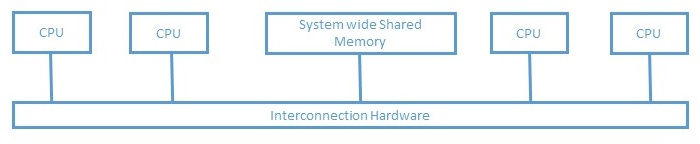
\includegraphics[width=10cm]{tightlyCoupledSystem}\\
            \caption{Tightly Coupled System}\label{tcs}
        \end{figure}
        \begin{figure}
            \centering
            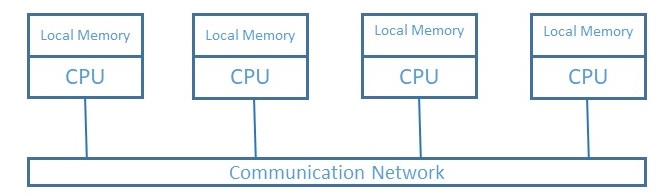
\includegraphics[width=10cm]{looselyCoupledSystem}\\
            \caption{Loosely Coupled System}\label{lcs}
        \end{figure}
    \end{frame}



\subsection{Evolution}\label{DCS}
    \begin{frame}
        \frametitle{Evolution of DCS}
            Content of Evolution
    \end{frame}



\subsection{DCS Models}
\begin{frame}
    \frametitle{Distributed Computing System Models}
    Various models are used for building distributed computing systems. These models can be broadly classified into five categories:
    \begin{itemize}
        \item {Minicomputer Model}
        \item {Workstation Model}
        \item {Workstation-Server Model}
        \item {Processor-Pool Model}
        \item {Hybrid Model}
    \end{itemize}
    \vspace{3cm}
\end{frame}



\subsection{Minicomputer Model}
\begin{frame}
    \frametitle{Minicomputer Model}
    \begin{figure}
        \centering
        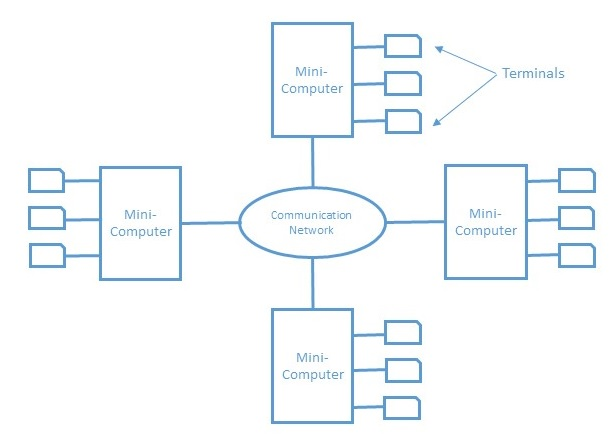
\includegraphics[width=10cm]{miniComputerModel}
        \caption{A DCS based on the Minicomputer Model}\label{minicomputermodel}
        \end{figure}
        \vspace{3cm}
\end{frame}



\subsection{Workstation Model}
\begin{frame}
    \frametitle{Workstation Model}
\begin{figure}
  \centering
  \includegraphics[width=7cm]{workStationModel}
  \caption{A DCS based on the Workstation Model}\label{workstationmodel}
\end{figure}

    Issues:
    \begin{itemize}
      \item {How does the system find an idle workstation?}
      \item {How is a process transferred from one workstation to another to get it executed?}
      \item {What happens to a remote process if a user logs onto a workstation that was idle until now and being used to execute a process of another workstation?}
    \end{itemize}
\end{frame}



\subsection{Workstation-Server Model}
\begin{frame}
    \frametitle{Workstation-Server Model}
    \begin{figure}
       \centering
       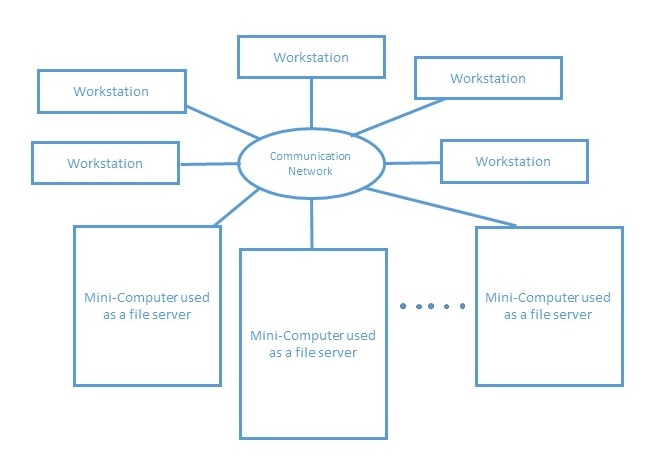
\includegraphics[width=10cm]{workStationServerModel}
       \caption{A DCS based on the Workstation-Server Model}\label{workstationservermocel}
    \end{figure}
    \begin{itemize}
      \item {Much Cheaper}
      \item {Diskless workstations are prefered to diskful workstations}
      \item {User have the flexibility to use any workstation and access the file in the same manner}
      \item {Request-response protocol is used to access the services of the machines}
      \item {A user has guaranted response time}
    \end{itemize}
    \vspace{1cm}
\end{frame}



\subsection{Processor-Pool Model}
\begin{frame}
    \frametitle{Processor-Pool Model}
    \begin{figure}[h!]
      \centering
      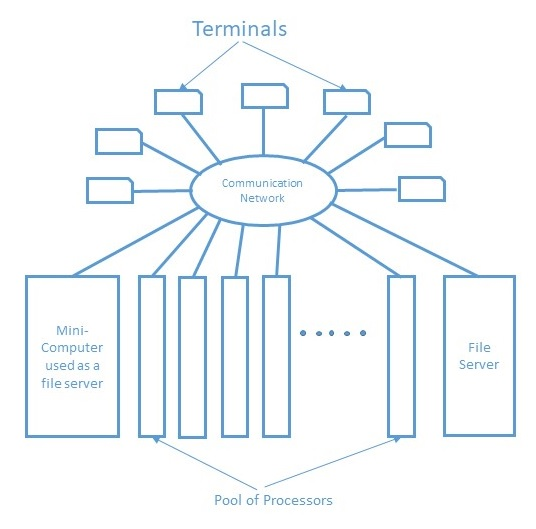
\includegraphics[width=7cm]{processorPoolModel}
      \caption{A DCS based on the Processor-Pool Model}\label{processorpoolmodel}
    \end{figure}
\end{frame}
\subsection{Hybrid Model}
\begin{frame}
    \frametitle{Hybrid Model}
\end{frame}



\subsection{Why are Distributed Systems Gaining Popularity?}
\begin{frame}
    \frametitle{Why are Distributed Systems Gaining Popularity?}
    Distributed Systems Gaining Popularity because...
    \begin{itemize}
      \item Inherently Distributed Applications
      \item Information Sharing among Distributed Users
      \item Resource Sharing
      \item better Price Performance Ratio
      \item Shorter Response Time and Higher Throughput
      \item Higher Reliability
      \item Extensibility and Incremental Growth
      \item Better Flexibility in Meeting User's Needs
    \end{itemize}
    \vspace{2cm}
\end{frame}



\subsection{What is DOS?}
\begin{frame}
    \frametitle{ What is Distributed Operating Systems?}
    \begin{itemize}
      \item What is Operating System?
        \\A program that controls the resources of a computer system and provides its user with an interface or a virtual machine that is more convenient to use than the bare machine. Therefor, primary tasks of OS are;
        \begin{itemize}
          \item To present users with a virtual machine that is easier to program than the underlying hardware.
          \item To manage the various resources of the system.
        \end{itemize}
        \vspace{1cm}
      \item Features:
      \begin{enumerate}
        \item System Image
        \item Autonomy
        \item Fault Tolerance Capability
      \end{enumerate}
    \end{itemize}
\end{frame}



\subsection{Issues}
\begin{frame}
    \frametitle{Issues In Designing a Distributed Operating System}
    \begin{enumerate}
		\item Transparency 
      	\item Reliability
      	\item Flexibility
      	\item Performance
      	\item Scalability
      	\item Heterogeneity
      	\item Security
      	\item Emulation of Existing System
    \end{enumerate}  
    \vspace{3cm} 
\end{frame}   


\begin{frame}[allowframebreaks]
    \frametitle{Issues In Designing a Distributed Operating System}
    \begin{enumerate}
      	\item {Transparency
      	\begin{enumerate}
      		\item Access Transparency
        	\item Location Transparency
        	\item Replication Transparency
        	\item Failure Transparency
        	\item Migration Transparency
        	\item Concurrency Transparency
        	\item Performance Transparency
        	\item Scaling Transparency
      	\end{enumerate}}
      	\vspace{4cm}
      	\framebreak
      	\item {Reliability
      	\begin{enumerate}
      		\item Fault Avoidance
      		\item Fault Tolerance
      		\item Fault Detection and Recovery
      	\end{enumerate}}
      	\vspace{6cm}
      	\framebreak
      	\item {Flexibility
      	\begin{enumerate}
      		\item Ease of Modification
      		\item Ease of Enhancement
      	\end{enumerate}}
      	\vspace{1cm}
      	The most important design factors that affects the flexibility of a distributed operating system is the model used for designing its kernel.Two commonly used models for kernel design in distributed operating system are;
      	\vspace{0.5cm}
      	\begin{itemize}
      		\item Monolithic Kernel Model
      		\item Microkernel Model
      	\end{itemize}
      	\framebreak
      	\begin{itemize}
      		\item Monolithic Kernel
      			\begin{figure}[h!]
      				\centering
      				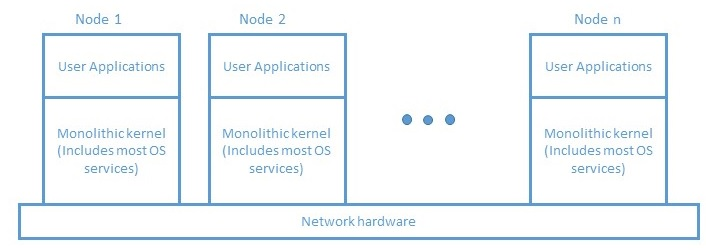
\includegraphics[width=10cm]{monoLithicKernelModel.jpg}
      				\caption{Monolithic Kernel Model}\label{monoLothicKernelModel}
      			\end{figure}
      			\vspace{1.5cm}
      			
      		\framebreak
      		\item Micro Kernel Model
      			\begin{figure}[h!]
      				\centering
      				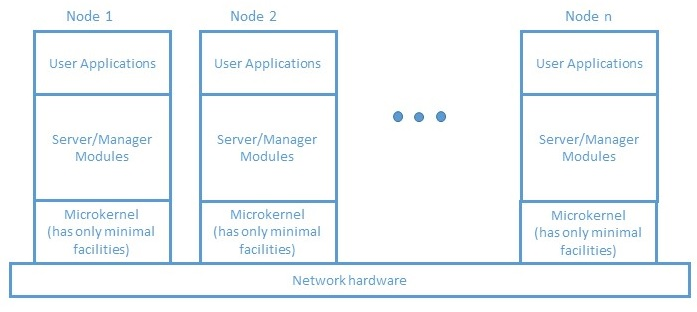
\includegraphics[width=10cm]{microKernelModel.jpg}
      				\caption{Monolithic Kernel Model}\label{microKernelModel}
      			\end{figure}
      			\vspace{1.5cm}
      	\end{itemize}
      	\vspace{6cm}
      	\framebreak
      	\item Performance\\
      		Some design principles considered useful for better performance as follows
      		\vspace{0.5cm}
      		\begin{itemize}
      			\item Batch if Possible
      			\item Cache whenever Possible
      			\item Minimize copying of Data
      			\item Minimize Network Traffic
      		\end{itemize}
      		\vspace{4cm}
      		\framebreak
      	\item Scalability\\
      		\vspace{0.5cm}
      		Some guiding principles for designing Scalable Distributed Operating Systems are as follows
      		\begin{itemize}
      			\item Avoid Centralized Entities
      			\item Avoid Centralized Algorithms
      			\item Perform Most Operations on Client Workstations
      		\end{itemize}
      		\vspace{1cm}
      	\item Heterogeneity
      	\item Security
    \end{enumerate}   
    \vspace{2cm}
\end{frame} 
\end{document}


